\documentclass[10pt,twocolumn,journal]{IEEEtran}
% XeLaTeX: all fonts are resolved from the local installation.
\usepackage{fontspec}
\defaultfontfeatures{Ligatures=TeX}
\setmainfont[
  BoldFont=TeXGyreTermes-Bold,
  ItalicFont=TeXGyreTermes-Italic,
  BoldItalicFont=TeXGyreTermes-BoldItalic,
  SmallCapsFont=TeXGyreTermes-Regular,
  SmallCapsFeatures={Letters=SmallCaps}
]{TeXGyreTermes-Regular}
\IfFontExistsTF{Arial}{\setsansfont{Arial}}{\setsansfont{Liberation Sans}}
\setmonofont{TeXGyreCursor-Regular}

\usepackage[margin=1in,bottom=1in]{geometry}
\usepackage{amsmath,amssymb}
\usepackage{booktabs,array,multirow}
\usepackage{graphicx}
\usepackage{xurl}
\usepackage{xr-hyper}
\usepackage[hidelinks]{hyperref}
\urlstyle{same}
\usepackage{fancyhdr}
\usepackage{flushend}
\externaldocument{supplement}[supplement.pdf]
\graphicspath{{figures/}}
\setlength{\emergencystretch}{4em}
\pagestyle{fancy}
\fancyhf{}
\fancyhead[L]{\scriptsize BELOW ZERO}
\fancyhead[R]{\scriptsize\thepage}
\renewcommand{\headrulewidth}{0pt}
\hypersetup{pdftitle={Below Zero: Spatially Adaptive Conditional Readout Sampling for Lower-Censored RAW Images},pdfauthor={},pdfsubject={Spatially adaptive conditional sampling of lower-censored RAW readouts}}
\newcommand{\BZAuthorBlockEN}{Yaogeng Jiang\\Independent Researcher\\\href{mailto:y.g.jiang@sjtu.edu.cn}{y.g.jiang@sjtu.edu.cn}}
\newcommand{\BZAuthorBlockZH}{姜尧耕\\独立研究者\\\href{mailto:y.g.jiang@sjtu.edu.cn}{y.g.jiang@sjtu.edu.cn}}
\newcommand{\BZPDFAuthors}{Yaogeng Jiang}

\hypersetup{pdfauthor={\BZPDFAuthors}}
\begin{document}
\title{{\normalsize \href{https://github.com/y-g-jiang/Video-RAW-Black-Level-Correction-Net/tree/main/below_zero}{Code and data}}\\[6pt]Below Zero: Spatially Adaptive\\Conditional Readout Sampling\\for Lower-Censored RAW Images}
\author{\BZAuthorBlockEN}
\maketitle
\thispagestyle{fancy}

\begin{abstract}
Clipping black-level-subtracted RAW measurements to zero discards negative readout codes and alters shadow statistics. We present a single-frame completion method that samples signed integers at censored positions while preserving every positive measurement. A multiscale convolutional estimator predicts the local signal, and a calibrated quantized Poisson--Gaussian decoder converts each prediction into probabilities for zero and negative codes. Reclipping the completed Bayer image exactly reproduces the input. On 138 held-out source images generated under a calibrated high-gain sensor model, N0/PG reduces excess Kullback--Leibler divergence from 0.001723 to 0.000313 nats relative to local likelihood estimation and improves realized-code negative log likelihood by 0.001407 nats per censored code. The KL improvement is observed for every source image. Regional analysis shows that classical estimators are already accurate near black, whereas larger gaps occur at higher signals and in nonuniform neighborhoods. Permuting the predicted laws without changing their collection increases error, revealing the importance of spatial assignment. Two real exposures with retained signed references show that neural and local conditional sampling both recover demosaicked shadow variation. These results establish a measurement-preserving approach to lower-censored RAW completion and quantify the contribution of learned spatial estimation to conditional readout accuracy.
\end{abstract}

\begin{IEEEkeywords}
Computational imaging, censored measurements, Bayer raw images, Poisson--Gaussian noise, probabilistic reconstruction, demosaicking.
\end{IEEEkeywords}

\section{Introduction and Related Work}
Black-level subtraction places RAW sensor measurements around a signed origin. Readout noise then produces negative codes in dark regions, even when the optical signal is nonnegative. Clipping these codes to zero changes the mean and variation of the observed noise \cite{foi2008,foi2009}, which can affect subsequent interpolation and averaging. Lower clipping appears in documented camera-processing pipelines \cite{mathworksISP}, camera-file investigations \cite{librawD5300,claffReadNoise}, and the clipped negative noise reported by the VMCL-ISP team in the AIM 2025 RAW-video challenge \cite{aim2025Video}. Nonnegative output constraints also arise in RAW-image evaluation interfaces \cite{sonyAIM2025}.

Our task is to complete a single lower-censored Bayer image with plausible signed readout samples. A zero observation merges an original quantized zero with every negative integer removed by clipping. The completion must fill these positions while leaving all positive measurements intact, thereby retaining the sensor-measurement representation used by later processing.

Identical observed zeros need not have identical conditional laws. A zero beside an illuminated structure provides different evidence about the missing readout than a zero in a uniformly dark patch. Nearby positive measurements provide signal evidence that a locally constant model can blur across structures. By estimating a spatial signal field, the same physical decoder can assign distinct readout distributions to the two locations.

N0/PG separates spatial estimation from conditional decoding. A NAF-style convolutional network \cite{nafnet} predicts a nonnegative signal field from the packed Bayer image and calibration parameters. A quantized Poisson--Gaussian (PG) decoder then evaluates the original integer readout distribution given the zero observation. The sampler fills only censored pixels, while an identity branch copies every positive code (Fig.~\ref{fig:pipeline}).

\begin{figure*}[t]
\centering
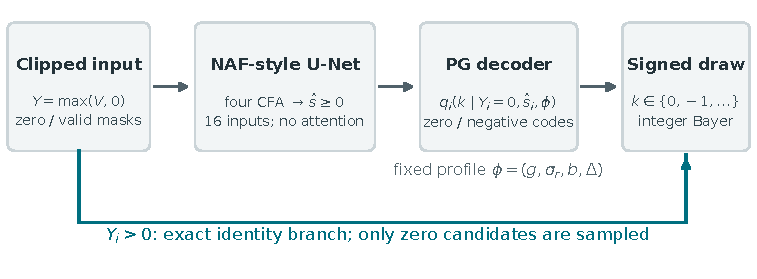
\includegraphics[width=\textwidth]{f01_pipeline.pdf}
\caption{Spatially adaptive signed-RAW completion. The network predicts a local signal parameter for the quantized PG decoder. Zero candidates are sampled from the resulting nonpositive integer law; observed positive codes pass through the identity branch unchanged.}
\label{fig:pipeline}
\end{figure*}

The central question is whether spatial context can improve the conditional readout law beyond local noise-model fitting. We test this on 138 held-out source images, analyze which scene structures account for the difference, and follow signed samples through demosaicking and a fixed color-rendering experiment.

\subsection{Related Work}
\subsubsection{Censored Measurements and RAW Noise Models}
Conditional imputation is a standard approach to censored observations. In Tobit regression, O'Neill \cite{oneill2024} uses latent-data augmentation to retain uncensored responses and draw censored responses from their conditional laws. In imaging, Kodgirwar et al. \cite{kodgirwar2024} infer saturated Poisson counts for multi-exposure ptychographic fusion. Our setting applies conditional readout completion to a single Bayer image with quantized PG noise, retaining the measured positive codes and the discrete probability of an original zero.

Foi et al. \cite{foi2008} developed a practical PG model for RAW noise, including clipping. Foi \cite{foi2009} then derived transformations and inverse corrections that permit denoising of clipped heteroskedastic observations. Their statistical model underlies our conditional decoder. Our output consists of sampled integer readouts at censored pixels, whereas their denoising objective estimates the latent signal. The Foi-qPG comparison applies those transformation and filtering methods before the same quantized conditional decoding used by the other estimators (Section~\ref{sec:baselines}).

Physical RAW noise also includes effects beyond independent Gaussian read noise. Wei et al. \cite{wei2020} model components relevant to extreme low light, Zhang et al. \cite{zhang2021} address correlated noise and quantization, and Mohammadi et al. \cite{mohammadi2026} examine biased black levels. These effects can change the missing negative-code distribution even when the measured zero and positive codes are unchanged.

\subsubsection{Learned Estimation and Conditional Sampling}
NAFNet \cite{nafnet} provides efficient convolutional blocks for image restoration. We use an independently implemented NAF-style encoder--decoder without pooled channel modulation, giving the estimator a finite spatial dependency. Its output is a signal parameter in DN; the calibrated PG model determines the associated probabilities.

Learned priors and measurement models meet in deep-equilibrium reconstruction \cite{gilton2021}, convex regularization \cite{goujon2023}, and Bayesian inversion with generative priors \cite{bohra2022}. Those approaches infer a latent image; here the unknown is a discarded integer readout conditioned on an observed zero. The Poisson-deconvolution study of Gnanasambandam et al. \cite{gnanasambandam2024} motivates examining individual estimator choices, while proper probability scores \cite{gneiting2007} assess the resulting conditional laws.

\subsubsection{Demosaicking and Downstream Processing}
Joint demosaicking and denoising use spatial and color correlations to recover clean images \cite{gharbi2016}. Our objective is earlier in the imaging chain: to restore plausible signed measurements before interpolation. We examine the effect of those measurements through adaptive homogeneity-directed (AHD) demosaicking \cite{hirakawa2005} with a specified LibRaw implementation \cite{libraw}.

\section{Conditional Readout Completion}
\subsection{A Quantized, Lower-Censored Readout}
Let $s_i\geq0$ be the expected optical signal in digital numbers (DN), $g$ the conversion gain in DN per electron, and $b_i$ a known offset relative to the nominal black level. Under the calibrated PG model, the photon count and continuous signed readout satisfy
\begin{align}
N_i&\sim\operatorname{Poisson}(s_i/g),\label{eq:pois}\\
Z_i&=gN_i+b_i+\epsilon_i,\qquad \epsilon_i\sim\mathcal N(0,\sigma_r^2).\label{eq:forward}
\end{align}
Nearest-integer quantization with a 1-DN step gives $V_i=\lfloor Z_i+1/2\rfloor$. We express the lower floor as zero after selecting a common signed-code origin; file-domain floors at other code values can be expressed by shifting that origin. Lower censoring then produces
\begin{equation}
Y_i=\max(V_i,0),\qquad \mathcal Z=\{i:Y_i=0\}.\label{eq:censor}
\end{equation}
The simulator includes upper saturation at $16383-512=15871$ DN. The evaluated samples remain above the physical lower ADC boundary; within this range, we use an unbounded Gaussian read-noise model.

For $k\leq0$, define the quantized mass
\begin{align}
a_k(s,b)=\sum_{n=0}^{\infty}\operatorname{Pois}(n;s/g)
\bigg[&\Phi\!\left(\frac{k+1/2-gn-b}{\sigma_r}\right)\nonumber\\[-2pt]
-&\Phi\!\left(\frac{k-1/2-gn-b}{\sigma_r}\right)\bigg],\label{eq:bin}
\end{align}
where $\Phi$ is the standard normal cumulative distribution function. The zero-observation probability is
\begin{equation}
c(s,b)=\sum_{n=0}^{\infty}\operatorname{Pois}(n;s/g)
\Phi\!\left(\frac{1/2-gn-b}{\sigma_r}\right).\label{eq:zeroevent}
\end{equation}
The $+1/2$-DN boundary includes both the quantization bin for the original zero and every negative-code bin.

Given a signal estimate $\hat s_i$, the decoder returns
\begin{equation}
q_i(k)=\frac{a_k(\hat s_i,b_i)}{c(\hat s_i,b_i)},\qquad k=0,-1,-2,\ldots.\label{eq:posterior}
\end{equation}
The bin integrals in \eqref{eq:bin} retain the discrete atom at $k=0$, while the normalization in \eqref{eq:posterior} conditions on the full zero-observation event. Fig.~\ref{fig:counterexamples} shows how the resulting law varies across image locations.

\subsection{Measurement-Preserving Completion}
For each candidate zero, draw $K_i$ from its predicted conditional law and construct
\begin{equation}
\widetilde V_i=\begin{cases}
Y_i,&Y_i>0,\\
K_i,\quad K_i\sim q_i,&Y_i=0.
\end{cases}\label{eq:output}
\end{equation}
The identity branch and nonpositive support of $q_i$ imply $\max(\widetilde V_i,0)=Y_i$ exactly. A conditional draw represents the missing readout variation, not a clean-signal estimate; a conditional mean and a random draw therefore serve different losses. We evaluate the predicted law with distribution scores, and derive the sample-versus-mean risk identities in Supplementary Section~I.

The simulator supplies the known-signal reference
\begin{equation}
p^{\star}_i(k)=a_k(s_i,b_i)/c(s_i,b_i)\label{eq:oracle}
\end{equation}
using the true $s_i$. At inference, the signal field is treated as fixed at $\hat s_i$, and $q_i$ describes the conditional readout variation. Pixelwise draws are independent given this estimated field.

\section{Learning Spatially Adaptive Readout Laws}
\subsection{Signal Estimator}
We pack the Bayer phases as $[R,G_1,G_2,B]$ and supply transformed measurements, zero indicators, known offsets, a validity mask, and calibration constants. The validity mask distinguishes padding from measured zeros; the offsets enter both the estimator and the PG decoder.

A NAF-style encoder--decoder combines four downsampling stages through additive skips and pixel-shuffle upsampling. Per-pixel normalization, depthwise convolutions, and multiplicative gates yield a finite spatial dependency without global pooling or attention. A four-channel softplus head predicts $\hat s_i\geq0$ in DN, and the decoder uses $\hat s_i/g$ as the electron mean. The model has 10,913,380 parameters; Supplementary Section~II gives the input channels and stage dimensions.

\subsection{Training With Conditional Distribution Targets}
Synthetic supervision supplies $s_i$ and the conditional target $p_i^\star$. We minimize cross entropy over valid zero candidates,
\begin{equation}
\mathcal L(\theta)=-\frac{1}{|\mathcal Z|}
\sum_{i\in\mathcal Z}\sum_{k\leq0}p^{\star}_i(k)\log q_{\theta,i}(k).
\label{eq:loss}
\end{equation}
The implementation evaluates \eqref{eq:loss} on a finite categorical representation with an explicit tail category. Its target entropy is constant with respect to the network, so minimizing the loss minimizes divergence from the known-signal target on that representation. Gradients pass through the physical decoder to the estimator, optimizing the signal prediction for conditional-distribution accuracy. Synthetic latent signals supply the targets and evaluation references. The decoder takes calibration parameters and per-realization offsets as known inputs; optimization updates only the spatial estimator.

\subsection{Numerical Law and Coordinate-Based Sampling}
The conditional law represents the individual codes $0,-1,\ldots,-304$ and one category for $V\leq-305$. The tail is resolved to individual integer codes when computing likelihoods and drawing samples. Supplementary Section~III describes the conditional tail calculation, numerical error bounds, and coordinate-keyed sampling.



\begin{figure*}[t]
\centering
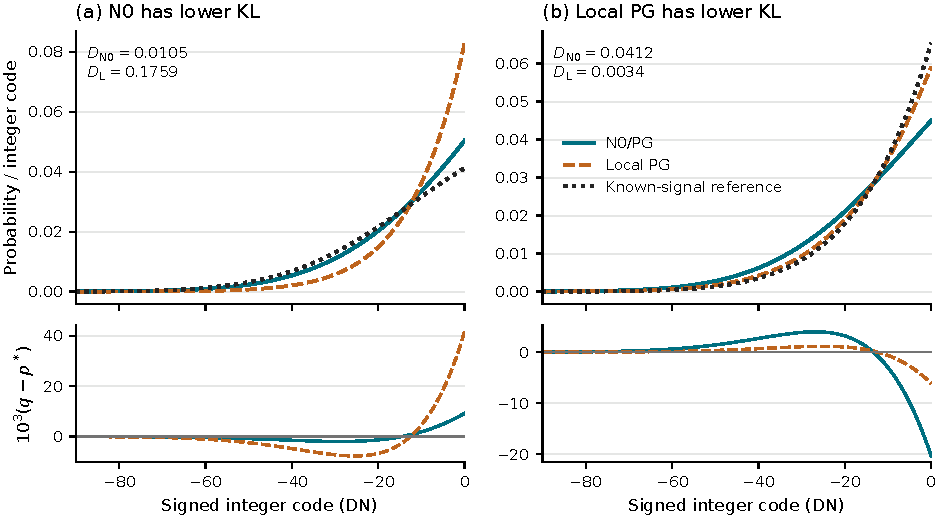
\includegraphics[width=\textwidth]{f02_pmf_counterexamples.pdf}
\caption{Conditional PMFs at two high-gradient development locations chosen after evaluation to illustrate opposite outcomes. Top: N0/PG, Local PG, and the known-signal law. Bottom: signed probability errors. N0 is more accurate in (a), while Local PG is more accurate in (b).}
\label{fig:counterexamples}
\end{figure*}

\section{Experiments}
\subsection{Data, Calibration, and Training}
The experiments use a calibrated Panasonic S5 II ISO12800 profile (Table~\ref{tab:protocol}). Gain comes from the JOT measurement \cite{jot}, and temporal read noise is estimated from ten dark frames using R/$G_1$. Synthetic signals, reference laws, and the conditional decoder share this PG model, so the held-out experiment tests spatial conditional-law estimation under matched noise assumptions; the retained real readouts evaluate the same model on real data.

\begin{table}[t]
\centering
\caption{Sensor calibration and experimental settings.}
\label{tab:protocol}
\small
\begin{tabular}{@{}p{0.40\columnwidth}p{0.52\columnwidth}@{}}
\toprule
Item & Setting\\
\midrule
Sensor setting & S5 II, ISO12800, mechanical shutter, 14 bit\\
Gain $g$ & 21.6010924121 DN/e$^{-}$\\
Integer read-noise RMS & 24.9612744275 DN\\
Analog $\sigma_r$ & 24.9596051193 DN\\
Nominal black level / step & 512 DN / 1 DN\\
Synthetic offset $b_c$ & Known; uniform $[-0.25,0.25]$ DN\\
Source-image split & 825 train / 137 dev / 138 test\\
Training & Seed 7103; 80,000 updates\\
Test contexts / target core & 128 and 256 / central 64 packed pixels\\
\bottomrule
\end{tabular}
\end{table}

The synthetic signal fields use 1,100 color-image templates from DIV2K and BSDS500 \cite{div2k,bsds500}, separated into 825 training, 137 development, and 138 test sources. The training distribution consists of 90\% natural scenes and 10\% procedural controls; exposure, color variation, quantization, and censoring follow the PG generator detailed in Supplementary Section~II. The single N0 checkpoint is selected on development data.

Each held-out source contributes two scenes with separately drawn exposure and noise, each evaluated with 128- and 256-pixel contexts sharing the central observations. This gives 552 cases and 3,254,612 scored entries, including 1,627,306 unique candidate locations in the 256-pixel context.






\subsection{Alternative Estimators}\label{sec:baselines}
Global PMF uses a training-derived average conditional law for each CFA phase. Global PG substitutes a training-derived per-phase signal into the calibrated decoder. Both provide spatially constant predictions at test time.

Local PG fits the signal in a same-CFA $5\times5$ window using the likelihood of observed positive codes and zero-censoring events. Local Bayes adds a fitted zero-plus-Gamma signal prior and integrates over the resulting conditional laws. Both use the same development-selected neighborhood; the center observation contributes once.

Foi-qPG adapts Foi's clipped-noise transformations \cite{foi2009} and BM3D filtering \cite{bm3d}, followed by a quantized-PG inverse mapping and the shared conditional integer decoder.

N0 estimates a multiscale signal field from all four CFA phases; the main local baselines use only same-CFA observations. A development-only Joint-CFA Bayes control also uses all phases but retains a locally constant-signal model (Supplementary Section~VII-A). It tests whether local cross-phase integration narrows the performance gap.

\subsection{Evaluation Criteria}
To assess the predicted conditional readout distributions, we score each withheld signed code $v_i$ using negative log likelihood and the discrete ranked probability score,
\begin{align}
\mathrm{NLL}(q_i,v_i)&=-\log q_i(v_i),\label{eq:nll}\\
\mathrm{CRPS}(q_i,v_i)&=\sum_{k\in\mathbb Z}
\left(F_{q_i}(k)-\mathbf{1}\{v_i\leq k\}\right)^2\Delta.\label{eq:crps}
\end{align}
NLL is measured in nats per candidate and CRPS in DN, with $\Delta=1$ DN. Both evaluate the actual withheld integer code, including values inside the resolved tail.

When the generating signal is known, we additionally compare the predicted law with the exact conditional law using excess KL and cumulative-distribution discrepancy,
\begin{align}
D_i&=\sum_{k\leq0}p^{\star}_i(k)\log\frac{p^{\star}_i(k)}{q_i(k)},\label{eq:kl}\\
J_i&=\sum_{k\in\mathbb Z}\left(F_{q_i}(k)-F_{p^{\star}_i}(k)\right)^2\Delta.\label{eq:cdf}
\end{align}
Excess KL and $J_{\mathrm{CDF}}$ use the common 306-category representation, including its coarsened tail. NLL and CRPS instead resolve individual tail codes. Supplementary Section~III specifies the corresponding numerical bounds.

Scores are averaged within source image and then equally across sources. Paired source-image bootstrap intervals preserve the related cases; the two designated KL comparisons against Local Bayes and Foi-qPG use 97.5\% intervals. Detailed aggregation and secondary analyses are specified in Supplementary Sections~\ref{sec:scoreaggregation} and~\ref{sec:regionaldefinitions}.

\subsection{Conditional-Law Accuracy on Held-Out Data}
N0/PG achieves the lowest excess KL, $J_{\mathrm{CDF}}$, NLL, and CRPS among the evaluated methods (Table~\ref{tab:holdout}). The known-signal law gives the attainable reference under the simulator, while zero filling cannot assign probability to the missing negative codes.

\begin{table*}[t]
\centering
\caption{Held-out conditional-distribution scores on 138 source images, each with four related case/context combinations. Scores use equal source weights. Excess KL and $J_{\mathrm{CDF}}$ use 306 categories; NLL and CRPS resolve the integer tail. Bold denotes the best deployable method. Zero fill assigns zero probability to negative labels, yielding infinite KL/NLL; the known-signal reference uses unavailable true signals.}
\label{tab:holdout}
\small
\begin{tabular}{@{}llrrrr@{}}
\toprule
Method & Available spatial information & $10^3D_{\mathrm{KL}}\downarrow$ & NLL$\downarrow$ & CRPS$\downarrow$ & $10^3J_{\mathrm{CDF}}\downarrow$\\
\midrule
Zero fill & None & $\infty$ & $\infty$ & 18.691235 & 10611.0233\\
Global PMF & Per-CFA training law & 3.4350 & 3.914828 & 8.112251 & 29.6469\\
Global PG & Per-CFA training signal & 3.3399 & 3.914723 & 8.111302 & 28.7879\\
Local PG & Same-CFA $5\times5$ & 1.7228 & 3.912975 & 8.095007 & 13.7075\\
Local Bayes & Same-CFA $5\times5$ & 1.8429 & 3.913102 & 8.096170 & 14.8024\\
Foi-qPG & Same-CFA image plane & 2.1475 & 3.913454 & 8.100521 & 18.5915\\
N0/PG (ours) & Four-CFA multiscale & \textbf{0.3125} & \textbf{3.911568} & \textbf{8.084118} & \textbf{2.6423}\\
Known-signal reference & Unavailable true signal & 0.0000 & 3.911245 & 8.081423 & 0.0000\\
\bottomrule
\end{tabular}
\end{table*}

The main KL differences, N0 minus Local Bayes and Foi-qPG, are $-1.5304\times10^{-3}$ and $-1.8350\times10^{-3}$ nats, with 97.5\% intervals $[-2.1085,-1.0776]\times10^{-3}$ and $[-2.1474,-1.5372]\times10^{-3}$. Relative to the local-likelihood estimator (Local PG), excess KL falls from $1.722793\times10^{-3}$ to $3.125067\times10^{-4}$ nats, an 81.86\% reduction.



The corresponding NLL improvement over Local PG is 0.001407 nats per candidate (95\% interval for N0 minus Local PG $[-0.001950,-0.000969]$), and CRPS decreases by 0.010890 DN (interval $[-0.014860,-0.007683]$). The much larger relative reduction in excess KL arises because expected log loss also contains the readout's irreducible conditional entropy. Fig.~\ref{fig:holdout} displays the absolute scores and paired differences.

The improvement is distributed across the test sources: N0 has lower KL than Local PG on all 138 images, lower NLL on 130, and lower CRPS on 131. The median source-wise KL reduction is $0.0004693$ nats.

\begin{figure*}[t]
\centering
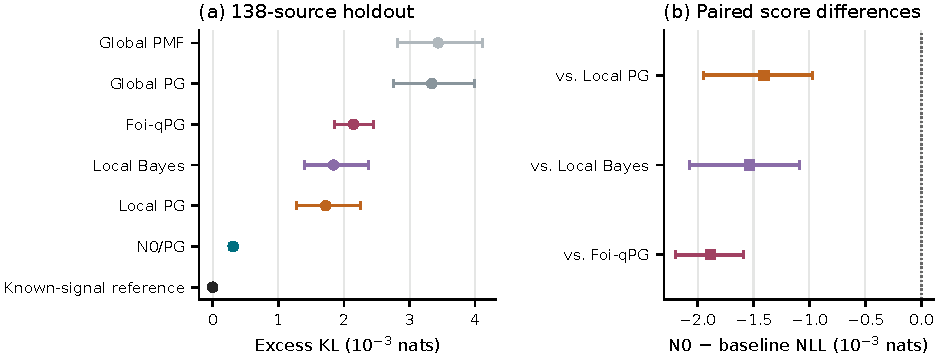
\includegraphics[width=\textwidth]{f03_holdout.pdf}
\caption{Held-out conditional-law accuracy. (a) Mean excess KL and 95\% source-bootstrap intervals. (b) Paired NLL differences with 95\% intervals; negative values favor N0. The primary 97.5\% intervals are reported in the text.}
\label{fig:holdout}
\end{figure*}

\subsection{Dependence on Signal and Neighborhood}\label{sec:regions}
The benefit of spatial estimation varies with signal and neighborhood structure. A zero close to a bright edge differs from one in a uniform dark region in both its underlying signal and its visible neighbors. We therefore examine the held-out conditional-law errors against signal strength, local variation, gradient distance, and the observed zero fraction (Fig.~\ref{fig:spatial}); bin definitions are in Supplementary Section~\ref{sec:regionaldefinitions}.

\subsubsection{Signal Level}
The near-black distribution is dominated by the calibrated read-noise tail, leaving little scope for disagreement among signal estimators. Accordingly, N0 minus Local Bayes has mean excess-KL difference $-0.000087$ nats at $s<0.25$ DN but $-0.002887$ nats at $8\leq s<16$ DN. Foi-qPG has lower mean error below 2 DN, while N0 has lower error above 4 DN (Fig.~\ref{fig:spatial}(a)).

\subsubsection{Neighborhood Variation}
Neighborhood structure is associated with a similar change. N0 minus Local Bayes is $-0.000358$ nats for $t<0.025$ and $-0.004467$ nats for $t\geq0.8$, across 379,366 and 98,229 candidates from 115 and 106 sources. The difference is $-0.002200$ nats at gradient locations, versus $-0.000330$ nats at distances of at least 16 packed pixels.

The observed zero fraction provides a complementary view: N0 minus Local Bayes is $-0.008058$ nats for $z<0.1$ (17,450 candidates) and $-0.000226$ nats for $0.5\leq z<0.75$ (498,135 candidates). The largest gap occurs when the censored pixel is surrounded mainly by positive observations. Signal level and neighborhood variation overlap, motivating the signal-matched development comparison in Section~\ref{sec:gradientcontrol}.

\begin{figure*}[t]
\centering
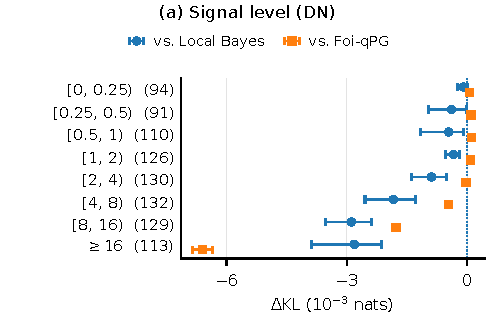
\includegraphics[width=0.493\textwidth]{f10a_holdout_signal.pdf}\hfill
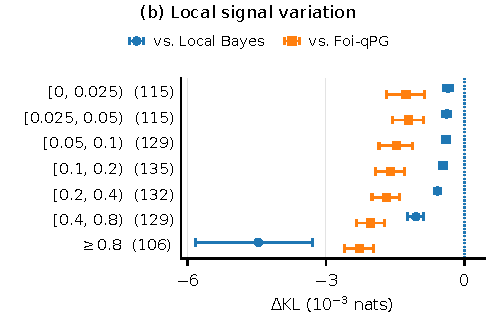
\includegraphics[width=0.493\textwidth]{f10b_holdout_variation.pdf}\\[1pt]
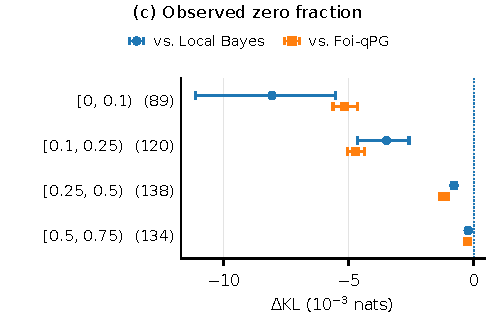
\includegraphics[width=0.493\textwidth]{f10c_holdout_zeros.pdf}\hfill
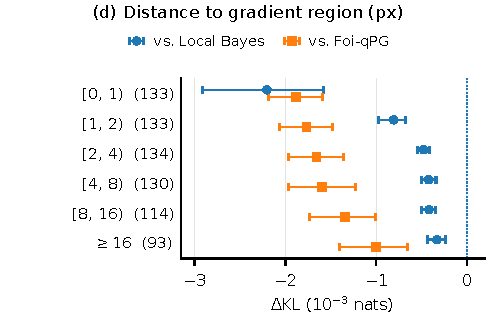
\includegraphics[width=0.493\textwidth]{f10d_holdout_gradient.pdf}
\caption{Regional error differences on the held-out test using the 256-pixel context. Points and 95\% source-bootstrap intervals show N0 minus Local Bayes (circles) or Foi-qPG (squares); negative values favor N0. Parentheses give source counts. Signal and gradient features in (a), (b), and (d) use simulated signals; zero fractions in (c) use the observed RAW. Bin definitions and counts are given in Supplementary Section~\ref{sec:regionaldefinitions}.}
\label{fig:spatial}
\end{figure*}

\subsection{Role of Spatial Information}
\subsubsection{Cross-CFA Information}
A local estimator can use all four CFA phases without adopting a multiscale signal field. On 32 development sources and 32,462 shared positions, this Joint-CFA Bayes estimator reaches excess KL 0.001790969, compared with 0.001952344 for same-CFA Local PG and 0.000376673 for N0 (Supplementary Table~\ref{tab:joint}). The result favors multiscale N0 over this particular local construction; the estimators also differ in spatial context and prior capacity.

\subsubsection{Location Assignment}
To separate the distribution of predictions from their spatial placement, we permute the predicted signals within each development source and CFA phase, keeping the calibration and the set of predicted laws unchanged.

This alone raises excess KL from 0.0003719 to 0.0026373 across 32 sources (assigned-minus-permuted $-0.0022654$, 95\% interval $[-0.0034895,-0.0012476]$). The result isolates a spatial effect: the same predicted laws score differently when attached to different pixels.

\subsubsection{Absolute Errors and Signal-Matched Contrasts}\label{sec:gradientcontrol}
Both estimators become less accurate around strong gradients, but Local PG deteriorates more. Across 32 development sources, the N0/Local PG excess KL changes from $0.000191/0.000791$ in low-gradient regions to $0.000442/0.002109$ in high-gradient regions. The source-wise high-minus-low contrast averages $-0.001066$ nats (median $-0.000102$, 23/32 sources below zero). Within-source, CFA- and signal-bin-matched comparison yields $-0.000268$ nats across 27 sources; its definitions and NLL results appear in Supplementary Section~IV.

\subsection{Calibration and Model Mismatch}
N0's 90\% equal-tail integer intervals cover 91.817\% of held-out codes, close to 91.853\% for the known-signal reference. Integer-valued intervals can contain more than their nominal mass; coverage assessed against that mass is reported at four nominal levels in Supplementary Table~\ref{tab:coverage}.





We also tested whether the advantage survives changes to the assumed noise. Across six development settings with perturbed read noise or additional unmodeled row/column offsets, N0 retains lower mean NLL and CRPS than Local PG. The size and uncertainty of each difference appear in Supplementary Fig.~\ref{fig:pairedstress}.

\subsection{Conditional Laws on Real Sensor Readouts}
Two 24-megapixel exposures, P2654748 and P2654749, retain signed sensor codes below the nominal black level. Phasewise integer shifts from independent dark frames define the hidden readout $V$; both methods receive the corresponding clipped image $Y=\max(V,0)$. The transformations and remaining fractional offsets appear in Supplementary Section~V.

Across six fixed regions per exposure, the R/$G_1$/$G_2$ scoring sets contain 12,652 and 19,200 censored positions. The B phase remains in the network input and sampled Bayer output, but its distinct sensor statistics make its real-data scores diagnostic only. Local estimators use $3\times3$ same-CFA neighborhoods in these cases.

\begin{table}[t]
\centering
\caption{Real signed-readout case studies. Each exposure uses shared R/$G_1$/$G_2$ candidates and the fixed real-data protocol. NLL is in nats per candidate and CRPS in DN; lower is better.}
\label{tab:real}
\footnotesize
\begin{tabular}{@{}lrrrr@{}}
\toprule
& \multicolumn{2}{c}{P2654748} & \multicolumn{2}{c}{P2654749}\\
\cmidrule(lr){2-3}\cmidrule(l){4-5}
Method & NLL & CRPS & NLL & CRPS\\
\midrule
Global PMF & 3.980276 & 8.289612 & 4.005568 & 8.347404\\
Global PG & 3.979631 & 8.283446 & 4.004966 & 8.341612\\
Local PG & 3.975846 & 8.248081 & 4.004176 & 8.331820\\
Local Bayes & 3.978475 & 8.273926 & 4.006270 & 8.352316\\
Foi-qPG & 3.979516 & 8.283580 & 4.006041 & 8.350880\\
N0/PG & \textbf{3.974503} & \textbf{8.237064} & \textbf{4.003213} & \textbf{8.322619}\\
\bottomrule
\end{tabular}
\end{table}

In P2654748 and P2654749, N0 improves NLL over Local PG by 0.001342 and 0.000964 nats, respectively, and CRPS by 0.011017 and 0.009200 DN. N0 has lower NLL in five of six ROIs in the first exposure and two of six in the second (Supplementary Section~\ref{sec:realcode} and the per-ROI results).

The calibrated PG law substantially underestimates the extreme negative tail. Among 31,852 candidates, $V\leq-128$, $V\leq-256$, and $V\leq-305$ DN occur 122, 21, and 13 times, compared with predicted counts of $9.01\times10^{-3}$, $3.76\times10^{-20}$, and $8.63\times10^{-30}$. The paired NLL differences remain in favor of N0 after excluding deep events or repeated coordinates (Supplementary Table~\ref{tab:real_robust}).



\subsection{Consequences for Demosaicking and Color}\label{sec:downstream}
\subsubsection{Real-Exposure Demosaicked Statistics}
To examine how completion affects a conventional imaging operation, we demosaic the retained signed reference, its clipped version, and samples from N0 and Local PG with the same AHD implementation. A common digital pedestal carries negative readouts through the unsigned LibRaw interface; we remove it in linear camera RGB before color processing.

For each of the 12 regions, we demosaic each of 32 conditional samples separately, compute its spatial statistics, and average those statistics over draws. In the darkest P2654748 region, clipping increases mean linear G from 9.003 to 16.322 DN; N0 and Local PG bring it to 8.621 and 8.602 DN. The spatial standard deviation of $R-G$ falls from 25.986 to 18.635 DN after clipping and returns to 25.157 DN with N0 and 25.256 DN with Local PG. Thus, conditional sampling recovers much of the shadow variation removed by censoring, with similar statistics for the two estimators. The two-exposure results are given in Supplementary Table~\ref{tab:ahd}.

The processing-order illustration and AHD implementation details are provided in Supplementary Section~V and \href{visual_en.pdf}{Supplementary Visual A}.

\subsubsection{Synthetic Clean-Reference Color Error}
A separate development experiment measures whether completing negative readouts affects dark-region color after rendering. Eight natural scenes and four procedural templates pass through AHD, fourfold signed-domain averaging, and fixed white balance, color conversion, and exposure. We measure squared error in the block-mean chroma vector $(R-G,B-G)$ against a quantized clean-signal reference in linear display RGB (Supplementary Section~\ref{sec:cleanendpoint}).

Direct clipping raises the natural-scene color error from 0.125006 for the signed readout to 1.257683. Conditional sampling brings it near the signed-reference level: 0.122891 with N0 and 0.126031 with Local PG. The N0-minus-Local difference is $-0.00314$ (95\% source-bootstrap interval $[-0.00614,-0.00084]$), a 2.49\% reduction across eight natural development sources. Quantized conditional means yield 0.102618 and 0.105440, respectively (Table~\ref{tab:cleanendpoint}); the four procedural scenes are reported separately.

\begin{table}[t]
\centering
\caption{Shadow-color error and clean-RAW MSE on eight natural development sources, with equal source weights. Color error is squared block-mean $(R-G,B-G)$ error in exposure-scaled linear display RGB. RAW MSE is measured against $Q(s)$ in DN$^2$. The signed input is the uncensored noisy readout. Lower is better for both metrics.}
\label{tab:cleanendpoint}
\small
\setlength{\tabcolsep}{4pt}
\begin{tabular}{@{}lrr@{}}
\toprule
RAW input & Dark-color error & RAW MSE\\
\midrule
Original signed & 0.125006 & 1157.747\\
Directly clipped & 1.257683 & \textbf{866.698}\\
Local PG sampled & 0.126031 & 1157.244\\
N0/PG sampled & \textbf{0.122891} & 1159.305\\
Local PG mean-$Q$ & 0.105440 & 1077.675\\
N0/PG mean-$Q$ & \textbf{0.102618} & 1076.179\\
\bottomrule
\end{tabular}
\end{table}

The two endpoints rank outputs differently. For any nonnegative clean reference $c=Q(s)$ and admissible fill $k\leq0$, $(k-c)^2-c^2=k^2-2kc\geq0$: with positive codes fixed, zero filling minimizes clean-RAW pixelwise MSE. Its change to shadow means nevertheless produces the largest block-color error in Table~\ref{tab:cleanendpoint}. Quantized conditional means give the lowest color error in this fixed rendering experiment.

\subsection{Runtime and Full-Resolution Inference}\label{sec:runtime}
A 24-megapixel signed completion takes 27.3901 s for N0/PG and 205.1503 s for Local PG on an RTX 3090 Ti, with peak allocated GPU memory of 750.69 and 94.84 MiB, respectively. These are measured implementations with different numerical backends; Supplementary Table~\ref{tab:runtime} gives the execution conditions.

Full-resolution inference uses overlapping phase-aligned tiles (Supplementary Section~VI). Coordinate-indexed sampling yields identical samples for a fixed law regardless of tile order (Supplementary Section~III).

\section{Discussion}
The held-out results connect conditional-law accuracy to the spatial placement of predicted readout distributions. Multiscale context is most useful around nonuniform signal structure, where the locally constant approximation is less accurate. Permuting the predictions among locations increases excess KL despite leaving their overall collection unchanged. The benefit therefore comes from assigning the conditional laws to suitable pixels as well as evaluating them with the PG decoder.

Distribution scores measure conditional readout accuracy, while downstream image statistics also depend on demosaicking and color processing. The matched-model experiment measures estimation error against a known-signal PG law. In the retained real exposures, the shared noise model substantially underestimates rare negative codes despite N0's small paired likelihood advantage. Both sampling methods recover some demosaicked shadow variation; the fixed-renderer development experiment further shows why zero filling can minimize clean-RAW MSE yet distort shadow colors.

These experiments characterize a single calibrated high-gain profile. The retained real readouts show that favorable aggregate scores can coexist with substantial rare-tail mismatch, motivating further tail calibration across sensor modes.

\section{Conclusion}
Lower-censored RAW zeros conceal a distribution of signed integer readouts. N0/PG estimates that law from surrounding Bayer measurements, samples only at censored positions, and preserves every positive code. On 138 held-out sources, the spatial laws outperform the evaluated local and transformed-domain estimators. Real signed readouts and a fixed-renderer development experiment illustrate their consequences for shadow statistics and color.

\section*{Reproducibility Statement}
The repository provides trained weights, inference and evaluation code, table-level scores, source identifiers, and color-evaluation records with SHA-256 manifests. The inference example was verified in an isolated environment. Original code and weights use MIT; original paper assets and numerical results use CC BY 4.0. Third-party terms are retained.

\section*{Acknowledgment}
OpenAI Codex and Kimi assisted with implementation, manuscript drafting, and language editing.

\bibliographystyle{IEEEtran}
\bibliography{references}
\end{document}
